% Created 2015-06-21 Dom 17:04
\documentclass[11pt]{article}
\usepackage[utf8]{inputenc}
\usepackage[T1]{fontenc}
\usepackage{fixltx2e}
\usepackage{graphicx}
\usepackage{longtable}
\usepackage{float}
\usepackage{wrapfig}
\usepackage{rotating}
\usepackage[normalem]{ulem}
\usepackage{amsmath}
\usepackage{textcomp}
\usepackage{marvosym}
\usepackage{wasysym}
\usepackage{amssymb}
\usepackage{hyperref}
\tolerance=1000
\usepackage{minted}
\usemintedstyle{perldoc}
\usepackage{tikz,enumerate}
\usetikzlibrary{decorations.markings}
\tikzstyle{vertex}=[circle, draw, inner sep=0pt, minimum size=7pt]
\providecommand{\vertex}{\node[vertex]}
\author{Alice Duarte Scarpa, Bruno Lucian Costa}
\date{2015-06-23}
\title{Exercício 8.19 (Tardos)}
\hypersetup{
  pdfkeywords={},
  pdfsubject={},
  pdfcreator={Emacs 24.4.1 (Org mode 8.2.10)}}
\begin{document}

\maketitle

\section{Enunciado}
\label{sec-1}

Um comboio de navios chega ao porto com um total de $n$ vasilhames
contendo tipos diferentes de materiais perigosos.
Na doca, estão $m$ caminhões, cada um com capacidade para até $k$
vasilhames.  Para cada um dos dois problemas, dê um algoritmo
polinomial ou prove NP-completude:


\begin{itemize}
\item Cada vasilhame só pode ser carregado com segurança em alguns
dos caminhões. Existe como estocar os $n$ vasilhames nos $m$
caminhões de modo que nenhum caminhão esteja sobrecarregado, e
todo vasilhame esteja num caminhão que o comporta com segurança?

\item Qualquer vasilhame pode ser colocado em qualquer caminhão,
mas alguns pares de vasilhames não podem ficar juntos num mesmo
caminhão. Existe como estocar os $n$ vasilhames nos $m$
caminhões de modo que nenhum caminhão esteja sobrecarregado e
que nenhum dos pares proibidos de vasilhames esteja no mesmo
caminhão?
\end{itemize}

\section{Item a}
\label{sec-2}

Uma solução força-bruta para esse problema seria:

\begin{itemize}
\item Estenda a lista de vasilhames com vasilhames vazios, até que ela
tenha tamanho $mk$ (a capacidade total de todos os
caminhões). Vasilhames vazios podem ser transportados em qualquer
caminhão (e correspondem a um lugar sobrando no mesmo).
\item Para cada uma das $(mk)!$ ordenações da lista acima, considere que
os $k$ primeiros vasilhames vão para o primeiro caminhão, os $k$
próximos para o segundo e assim até o final da lista. Se cada
vasilhame estiver em um camihão que o comporta com segurança,
retorne essa solução, se não, tente com uma nova ordem.
\end{itemize}

Esse algoritmo faz $(mk)!$ iterações do loop principal no pior caso, cada
iteração tem custo $mk$ para conferir se é uma solução válida. Isso dá
uma complexidade total de $O(mk(mk)!)$

Esse é um algoritmo super-exponencial para o problema, mas isso não
significa que o problema é NP-completo. Na verdade, como veremos a
seguir, esse problema não é NP-completo pois aceita uma solução
polinomial usando fluxos.

\subsection{Solução com fluxos}
\label{sec-2-1}

Podemos transformar esse problemas em um problema de encontrar o fluxo
máximo de um grafo usando a seguinte construção:

\begin{itemize}
\item Criamos um vértice $s$ representando a fonte e um vértice $t$
  representando o dreno

\item Para cada vasilhame $v_i \in \{v_1, v_2, \ldots, v_n\}$ criamos um
vértice $v_i$ e uma aresta $(s, v_i)$ capacidade 1

\item Para cada caminhão $C_i \in \{C_1, C_2, \ldots, C_m\}$ criamos um
vértice $C_i$. Se o vasilhame $v_j$ puder ser transportado com
segurança no caminhão $C_i$ criamos uma aresta $(v_j, C_i)$ de
capacidade 1. Para cada caminhão criamos também uma aresta $(C_i, t)$
de capacidade $k$.
\end{itemize}

Dessa forma, existe uma configuração possível de caminhões se e
somente se o fluxo máximo tem valor $m$.

De fato, se encontramos um fluxo máximo de valor $m$ então exatamente
uma aresta com origem em cada vasilhame terá fluxo 1. Se colocarmos
cada vasilhame no caminhão de destino da aresta de fluxo 1 obtemos um
posicionamento válido. Por outro lado, se existe um arranjo válido,
colocando 1 de fluxo nas arestas entre os vasilhames e os caminhões
que os contém nesse arranjo obtemos um fluxo de valor $m$.

Para a seguinte situação:
\begin{center}
\begin{tabular}{lr}
Capacidade & 3\\
Total de cam. & 4\\
Total de vas. & 10\\
\end{tabular}
\end{center}


\begin{center}
\begin{tabular}{r l}
Vasilhame & Cam. seguros\\
1 & 1, 4\\
2 & 1, 2\\
3 & 3, 4\\
4 & 4\\
5 & 1, 2, 3, 4\\
6 & 1\\
7 & 3\\
8 & 1, 2, 3\\
9 & 2, 3\\
10 & 4\\
\end{tabular}
\end{center}



A construção seria como ilustrado na figura abaixo. Omitimos as
capacidades iguais a 1 para não poluir demais a imagem.

\[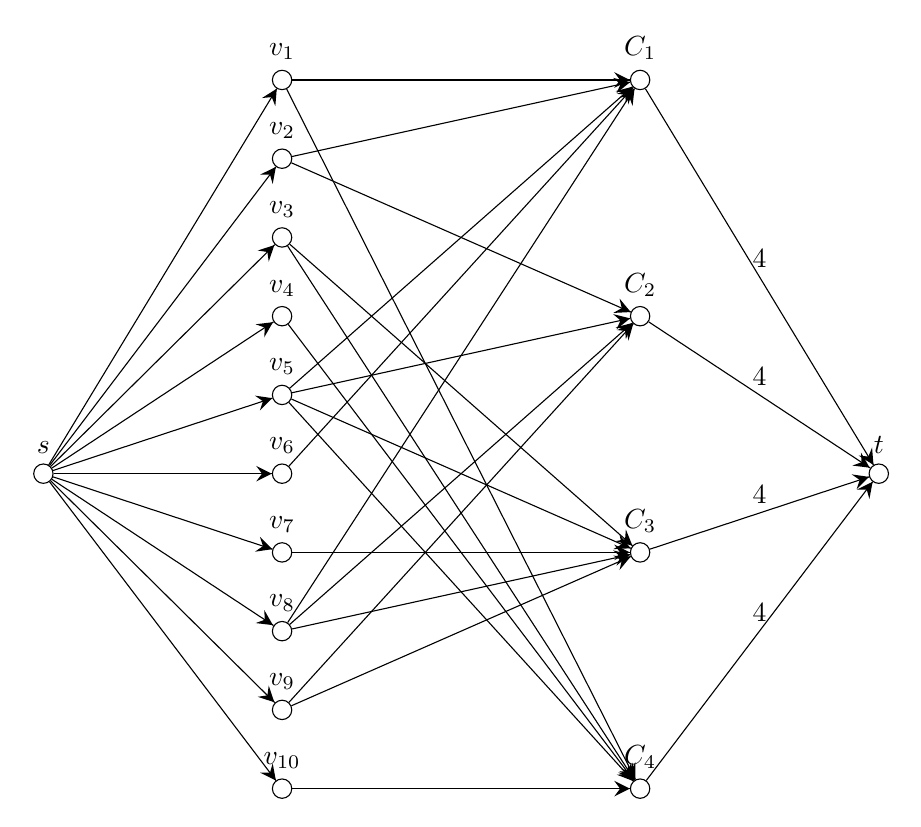
\begin{tikzpicture}[x=0.25\textwidth,
    every edge/.style={
        draw,
        postaction={decorate,
                    decoration={markings,mark=at position 1 with {\arrow[line width = 0.5mm]{stealth}}}
                   }
        }
]
\vertex (fonte) at (0,5) [label=above:$s$] {};
\vertex (v1) at (1,10) [label=above:$v_1$] {};
\vertex (v2) at (1,9) [label=above:$v_2$] {};
\vertex (v3) at (1,8) [label=above:$v_3$] {};
\vertex (v4) at (1,7) [label=above:$v_4$] {};
\vertex (v5) at (1,6) [label=above:$v_5$] {};
\vertex (v6) at (1,5) [label=above:$v_6$] {};
\vertex (v7) at (1,4) [label=above:$v_7$] {};
\vertex (v8) at (1,3) [label=above:$v_8$] {};
\vertex (v9) at (1,2) [label=above:$v_9$] {};
\vertex (v10) at (1,1) [label=above:$v_{10}$] {};
\vertex (C1) at (2.5,10) [label=above:$C_1$] {};
\vertex (C2) at (2.5,7) [label=above:$C_2$] {};
\vertex (C3) at (2.5,4) [label=above:$C_3$] {};
\vertex (C4) at (2.5,1) [label=above:$C_4$] {};
\vertex (dreno) at (3.5,5) [label=above:$t$] {};
\path
(fonte) edge (v1)
(fonte) edge (v2)
(fonte) edge (v3)
(fonte) edge (v4)
(fonte) edge (v5)
(fonte) edge (v6)
(fonte) edge (v7)
(fonte) edge (v8)
(fonte) edge (v9)
(fonte) edge (v10)
(v1) edge (C1)
(v1) edge (C4)
(v2) edge (C1)
(v2) edge (C2)
(v3) edge (C3)
(v3) edge (C4)
(v4) edge (C4)
(v5) edge (C1)
(v5) edge (C2)
(v5) edge (C3)
(v5) edge (C4)
(v6) edge (C1)
(v7) edge (C3)
(v8) edge (C1)
(v8) edge (C2)
(v8) edge (C3)
(v9) edge (C2)
(v9) edge (C3)
(v10) edge (C4)
(C1) edge node [above] {$4$} (dreno)
(C2) edge node [above] {$4$} (dreno)
(C3) edge node [above] {$4$} (dreno)
(C4) edge node [above] {$4$} (dreno)
;
\end{tikzpicture}\]

\subsubsection{Implementação}
\label{sec-2-1-1}

Primeiramente, precisamos ser capazes de ler a tabela acima para
passar os valores para o nosso algoritmo.
\begin{minted}[]{python}
capacidade_por_caminhao = regras[0][1]
total_de_vasilhames = regras[2][1]
\end{minted}

\begin{minted}[]{python}
vasilhames = collections.OrderedDict()
caminhoes = []
for line in seguros[1:]:
    # Nomeando os vasilhames
    vasilhame = 'v_%s' % line[0]
    vasilhames[vasilhame] = []
    for caminhao in str(line[1]).split(','):
        nome = 'C_%s' % caminhao.strip()
        vasilhames[vasilhame].append(nome)
        if nome not in caminhoes:
            caminhoes.append(nome)
\end{minted}

Vamos usar a classe RedeDeFluxo, que definimos para a questão 7.28.

\begin{minted}[]{python}
def cria_grafo(vasilhames, caminhoes, capacidade_por_caminhao):
    G = RedeDeFluxo()
    G.novo_vertice('Fonte')
    G.novo_vertice('Dreno')

    # Criando um vertice para cada caminhao e ligando esse vertice ao dreno
    for caminhao in caminhoes:
        G.novo_vertice(caminhao)
        G.nova_aresta(caminhao, 'Dreno', capacidade_por_caminhao, 0)

    for vasilhame, caminhoes in vasilhames.iteritems():
        # Criando um vertice para cada vasilhame e conectando a fonte a
        # cada um dos vasilhames
        G.novo_vertice(vasilhame)
        G.nova_aresta('Fonte', vasilhame, 1, 0)

        # Conectando o vasilhame a cada caminhao que pode transporta-lo
        for caminhao in caminhoes:
            G.nova_aresta(vasilhame, caminhao, 1, 0)

    return G
\end{minted}

Como nesse problema as demandas já são 0, podemos aplicar
Ford-Fulkerson diretamente, usando a mesma implementação que fizemos
para o exercício 7.28.

Podemos então rodar Ford-Fulkerson e ver se o fluxo máximo encontrado
é igual ao total de vasilhames. Se for, isso significa que o problema
tem uma solução, que vamos retornar. Caso contrário não existe arranjo
possível.
\begin{minted}[]{python}
G = cria_grafo(vasilhames, caminhoes, capacidade_por_caminhao)
fluxo = G.fluxo_maximo('Fonte', 'Dreno')
if fluxo == total_de_vasilhames:
    tabela_de_vasilhames = []
    for vasilhame in vasilhames:
        for w in G.adj[vasilhame]:
            if G.fluxo[w] == 1:
                tabela_de_vasilhames.append([w.origem, w.destino])
    return tabela_de_vasilhames
else:
    return 'Impossivel'
\end{minted}

A solução para a nossa entrada:
\begin{center}
\begin{tabular}{ll}
v$_{\text{1}}$ & C$_{\text{4}}$\\
v$_{\text{2}}$ & C$_{\text{2}}$\\
v$_{\text{3}}$ & C$_{\text{3}}$\\
v$_{\text{4}}$ & C$_{\text{4}}$\\
v$_{\text{5}}$ & C$_{\text{1}}$\\
v$_{\text{6}}$ & C$_{\text{1}}$\\
v$_{\text{7}}$ & C$_{\text{3}}$\\
v$_{\text{8}}$ & C$_{\text{1}}$\\
v$_{\text{9}}$ & C$_{\text{2}}$\\
v$_{\text{10}}$ & C$_{\text{4}}$\\
\end{tabular}
\end{center}

\subsubsection{Complexidade}
\label{sec-2-1-2}

Como vimos no exercício 7.28, O algoritmo de Ford-Fulkerson tem
complexidade $O((V + E)F)$ em que $V$ é a quantidade de vértices, $E$
é a quantidade de arestas e $F$ é o maior valor possível para o fluxo.

No caso, $V = m + n + 2$, $E \leq n + nm + m$ e o maior fluxo possível é
$n$, totalizando uma complexidade máxima $O(n^2m)$, o que é polinomial na
entrada.

\section{Item B}
\label{sec-3}

Vamos mostrar que é possível reduzir uma instância do 3-SAT a um
problema de colocar vasilhames em caminhões seguindo as restrições do
enunciado. De modo que, como 3-SAT é NP-completo, nosso problema
também é.

\subsection{Definindo 3-SAT}
\label{sec-3-1}

3-SAT é o problema de dado um conjunto de variáveis $v_1, \ldots, v_x$
e cláusulas $K_1, \ldots, K_y$, onde cada cláusula é constituída de no
máximo três elementos do universo de \textit{literais}, $\{v_1,
\overline{v_1}, \ldots, v_x, \overline{v_x}\}$, encontrar uma
atribuição de valores Verdadeiro/Falso para cada variável
que faça com que todas as cláusulas sejam verdadeiras.

\subsection{3-SAT $\to$ Caminhões}
\label{sec-3-2}

Dada uma instância do 3-SAT, vamos construir uma instância do problema
enunciado que admite solução se e somente se tal
instância do 3-SAT admite solução.

Primeiramente, note que podemos assumir que nosso
problema de 3-SAT tem pelo menos quatro variáveis, adicionando
variáveis que não aparecem em cláusula alguma se necessário.

\subsubsection{Construção}
\label{sec-3-2-1}

Vamos começar a construção sem as cláusulas:

\begin{itemize}
\item São $x+1$ caminhões, cada um de capacidade $3x+y$

\item Existe um vasilhame para cada um dos $2x$ literais em $\{v_1,
  \overline{v_1}, \ldots, v_x, \overline{v_x}\}$. Esses vasilhames têm o
mesmo nome do literal a que correspondem.

\item Existe um vasilhame adicional $w_i$ para cada variável $v_i$
\end{itemize}

Queremos criar restrições entre os vasilhames de modo que, em uma
atribuição válida:

\begin{enumerate}
\item $x$ dos caminhões contenham exatamente um literal verdadeiro cada.
\item O caminhão restante contenha todos os literais falsos;
\end{enumerate}

Para garantir as condições acima, vamos criar os seguintes conflitos:
\begin{itemize}
\item $w_i$ conflita com $w_j$ para todo $i \neq j$.
\item $w_i$ e conflita com $v_j$ e com $\overline{v_j}$, se $i \neq j$.
\item $v_i$ conflita com $\overline{v_i}$.
\end{itemize}

Com isso, garantimos as seguintes propriedades:

\begin{enumerate}[($P_1$)]
\item Como todos os $w_i$ conflitam entre si, é necessário um
caminhão por $w_i$.

\item Como $w_i$ conflita com todos os literais tais que
$i \neq j$, o caminhão que contém $w_i$ só pode conter literais
correspondentes a $i$-ésima variável.

\item $v_i$ e $\overline{v_i}$ não
podem estar ambas no caminhão do $w_i$, pois elas conflitam entre si.

\item Mais ainda, $\textit{exatamente}$ um elemento do par $\{v_i,
\overline{v_i}\}$ está no caminhão do $w_i$ numa atribuição válida: Se
nenhuma delas estivesse no caminhão do $w_i$, estariam ambas no único
caminhão que não contém nenhum $w$ (pois todos os outros caminhões
contém um $w_j$ com $i \neq j$, o que conflita com $v_i$ e
$\overline{v_i}$), o que também não pode acontecer.
\end{enumerate}



Agora, vamos adicionar as cláusulas à nossa construção:

\begin{itemize}
\item Existe um vasilhame para cada uma das $y$ cláusulas $K_1, \ldots, K_y$
\end{itemize}

Com seguinte conflito:

\begin{itemize}
\item $K_i$ conflita com $v_j$ se $v_j \not\in K_i$. Similarlmente, $K_i$
  conflita com $\overline{v_j}$ se $\overline{v_j} \not\in K_i$.
\end{itemize}

Ou seja, permitimos colocar o vasilhame da cláusula $K_i$ num caminhão
apenas se a cláusula contém todos os literais que vão viajar no
caminhão.

Dessa forma, uma cláusula nunca pode viajar no caminhão dos literais
falsos, pois cada a cláusula contém no máximo três literais e temos no
mínimo quatro literais falsos, de modo que há garantidamente um
literal que não aparece na cláusula e portanto conflita com ela.

\subsubsection{Obtendo uma solução}
\label{sec-3-2-2}

Para completar a nossa redução, precisamos de duas coisas:
\begin{itemize}
\item A partir de uma solução do problema dos caminhões que construimos,
encontrar em tempo polinomial uma solução do 3-SAT correspondente
\item Provar que quando nenhuma solução do problema dos caminhões existe o
3-SAT também não tem solução
\end{itemize}

\begin{enumerate}
\item Solução caminhões $\to$ Solução 3-SAT
\label{sec-3-2-2-1}

Se existe uma solução para o problema, então todo caminhão que contém
um vasilhame do tipo $w_i$ também contém um vasilhame correspondente a
um literal, pela propriedade $P_4$; esse literal será marcado como
verdadeiro. Todos os outros literais serão marcados como falsos. Essa
marcação é consistente, pois para cada $i \in \{1, 2, \ldots, x\}$
exatamente um literal entre $v_i, \overline{v_i}$ que está no mesmo
caminhão que $w_i$. Como todas as cláusulas têm que estar em um
caminhão que contém um vasilhame do tipo $w_i$ e esse caminhão tem que
conter um literal que está na cláusula, essa marcação faz com que
todas as cláusulas sejam verdadeiras.


\item $\not \exists$ solução caminhões $\Rightarrow \not \exists$ solução 3-SAT
\label{sec-3-2-2-2}

É mais fácil provar a contrapositiva, isso é, $\exists$ solução 3-SAT
$\Rightarrow \exists$ solução caminhões.

Seja $S$ os conjuntos dos literais verdadeiros na solução do 3-SAT.
Então:
\begin{itemize}
\item $S \subset \{v_1,\overline{v_1}, \ldots, v_x, \overline{v_x}\}$
\item $\forall \; 1\leq i \leq x, |S\cap\{v_i, \overline{v_i}\}| = 1$
\item $\forall \; 1\leq j \leq y, S\cap K_j \neq \emptyset$
\end{itemize}

Podemos construir uma solução válida para o problema dos caminhões da
seguinte forma:
\begin{itemize}
\item $\forall \; 1\leq i \leq x$, coloque o vasilhame $w_i$ no caminhão $C_i$
\item $\forall \; 1\leq i \leq x$, coloque o vasilhame $S\cap\{v_i, \overline{v_i}\}$ em $C_i$
\item $\forall \; 1\leq j \leq y$, seja $i$ o menor valor tal que $v_i$ ou
$\overline{v_i}$ está em $S\cap K_j$. Coloque o vasilhame $K_j$ em $C_i$.
\item Coloque todos os literais em $\{v_1,\overline{v_1}, \ldots, v_x,
  \overline{v_x}\} - S$ no caminhão $C_{x+1}$
\end{itemize}


Isso respeita todas as restrições. De fato, cada $K_j$ está num
caminhão que só contém um vasilhame correspondente a um literal e,
pelo item 3, o vasilhame do literal não conflita com o vasilhame da
cláusula. Além disso, cada $w_i$ está em seu próprio caminhão, nenhum
par $\{v_i, \overline{v_i}\}$ aparece num mesmo caminhão e nenhum
$w_i$ aparece no mesmo caminhão de um literal $v_j$ ou
$\overline{v_j}$ com $i \neq j$.
\end{enumerate}
% Emacs 24.4.1 (Org mode 8.2.10)
\end{document}
